% Results section

The section will outline the major results of the clustering. 
It is focused on the broad band clustering, and two combinations from the narrow band colours.
The first narrow band combination is the most successful narrow band clustering, and the second is the least successful.
A complete discussion of all the combinations can be found in Appendix 1 \textbf{Make appendix here}.

% BROAD BAND CLUSTERINGS ----------------------------------------------
\subsection{Broad - Broad Band Combinations}
Table~\ref{tab:BBcolours} lists the broad band combinations that were clustered. 
In both two and three dimensions, the $U - B$ and $V - I$ combination was clustered more effectively than the $U - V$ and $B - I$ combination, and will be the combination used for discussion.

\subsubsection{2-Dimensions}
The two dimensional clustering was successful in identifying features within the distribution, however, it's segmentation was not as strong as the three dimensional clustering. 
% Broad band table
%\begin{landscape}
\begin{table*}
\centering
\caption{Summary of $U - B$ and $V - I$ combination two dimensional clusterings.}
\label{tab:BBclustering}
\begin{tabular}{llllllllllll}
\hline\hline
Method & Clusters & Parameters & Score & Cluster 1 & Cluster 2  & Cluster 3 & Cluster 4 & Cluster 5 & Cluster 6 & Cluster 7 & Cluster 8\\
\hline
K-Means & 3 & $K = 3$ & 0.4413 & 2215 & 7892 & 18824 & $ - $ & $ - $ & $ - $ & $ - $ & $ - $ \\
K-Means & 4 & $K = 4$ & 0.3741 & 2590 & 12924 & 2034 & 11383 & $ - $ & $ - $ & $ - $ & $ - $ \\
K-Means & 5 & $K = 5$ & 0.3577 & 7541 & 1513 & 5472 & 2298 & 12107 & $ - $ & $ - $ & $ - $ \\
K-Means & 6 & $K = 6$ & 0.3271 & 986 & 1618 & 5237 & 8373 & 8149 & 4568 & $ - $ & $ - $ \\
K-Means & 7 & $K = 7$ & 0.3254 & 4512 & 2371 & 999 & 6862 & 7283 & 1047 & 5857 & $ - $ \\
K-Means & 8 & $K = 8$ & 0.3186 & 2733 & 4437 & 5737 & 5091 & 6705 & 2455 & 684 & 1089 \\
Meanshift & 8 & $h = 0.4000 $ & 0.4236 & 25308 & 2518 & 48 & 6 & 57 & 917 & 1 & 76 \\
Meanshift & 5 & $h = 0.4500 $ & 0.3981 & 28074 & 533 & 9 & 1 & 314 & $ - $ & $ - $ & $ - $ \\
Meanshift & 5 & $h = 0.5000 $ & 0.3962 & 28129 & 487 & 9 & 305 & 1 & $ - $ & $ - $ & $ - $ \\
Meanshift & 5 & $h = 0.5500 $ & 0.4037 & 27927 & 706 & 9 & 1 & 288 & $ - $ & $ - $ & $ - $ \\
\hline
\end{tabular}
\end{table*}
%\end{landscape}
Table~\ref{tab:BBclustering} summarzies the results of the two dimensional clusterings.
This table lists the parameters that produced the clusterings, and the number of objects in each cluster.

\paragraph{K-Means}
The optimal clustering selected was at $K=5$ (Figure~\ref{fig:BB2dKM5} as it is the point where the score begins to plateau.
K-Means performed more effectively than Meanshift in 2-dimensions.
K-Means was able to identify the branch of red $U - B$ objects at low values of $K$.
As $K$ increased, the algorithm was also able to identify a group of objects that are red in $V - I$, and blue in $U - B$. 

\begin{figure}[H]
\centering
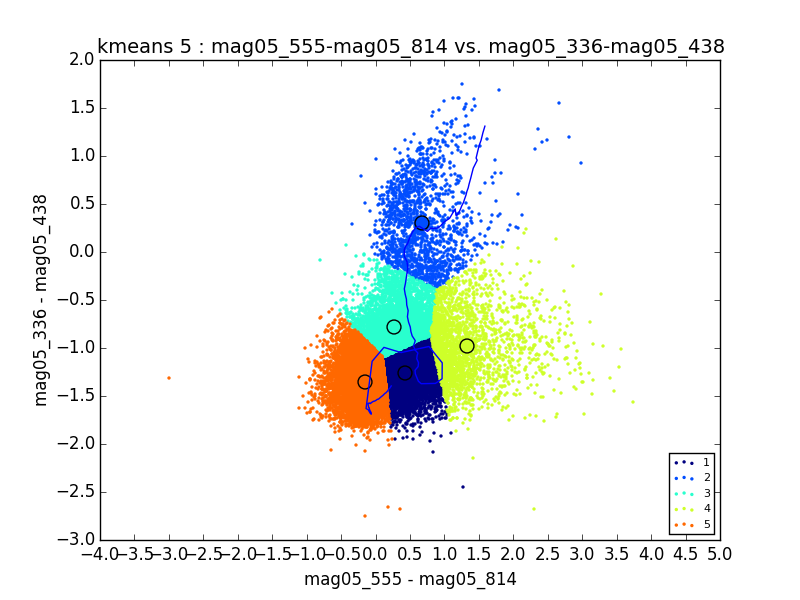
\includegraphics[width=\linewidth]{figs/broad/kmeans_color_5cl_mag05_555-mag05_814vsmag05_336-mag05_438}
\caption{Colour-Colour distribution of the $U - B$ and $V - I$ colours, clustered using K-Means with $K=5$. The colour of each point corresponds to the cluster the point was assigned to. Cluster numbers can be seen in the legend.}
\label{fig:BB2dKM5}
\end{figure}

The boundaries of each cluster approximately represent integers in each colour, and identify groups of objects that are relatively blue and red, seperating them from objects with extremes of either colour.
\textbf{Discuss statistics here}
The clusters trace sections of the modelled colours. 
The centers of clusters 2 and 5 line up well with the models, indicating that these clusters could be representative of different ages of objects in this distribution.
\textbf{Not sure if that was the right implication or if there is something else to their alignment}. 

\paragraph{Meanshift}
The optimal Meanshift clustering was selected as the point where the bandwidth converged, and can be seen in Figure~\ref{fig:BB2dMS5}.
Its bandwidth was $h=0.6$, which produced five clusters.

\begin{figure}[H]
\centering
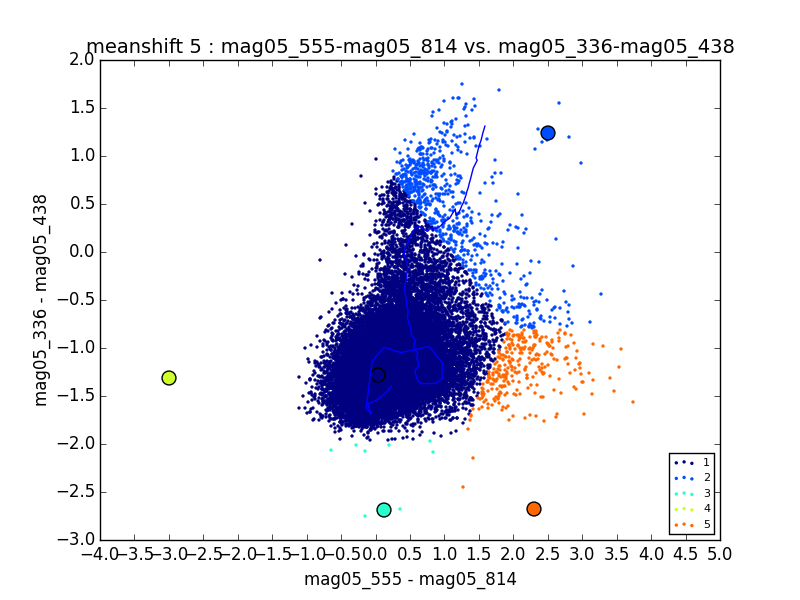
\includegraphics[width=\linewidth]{figs/broad/meanshift_color_5cl_mag05_555-mag05_814vsmag05_336-mag05_438}
\caption{Colour-Colour distribution of the $U - B$ and $V - I$ colours, clustered using Meanshift with $h=0.6$ producing five clusters. The colour of each point corresponds to the cluster the point was assigned to. Cluster numbers can be seen in the legend.}
\label{fig:BB2dMS5}
\end{figure}

This clustering was not as strong as K-Means, as it failed to identify the branch of red objects (cluster 2 in Figure ~\ref{fig:BB2dKM5}) that is a major feature of the distribution.
Additionally, the clusters and their centers do not align with the model colours, indicating that Meanshift was unable to identify different segments of the stellar lifecycle.
\textbf{Add cluster statistics here}.

\paragraph{Clustering Comparison}
Figure~\ref{fig:BB2dMSKMcomp} shows the comparison between the two optimal clusterings.

\begin{figure}[H]
\centering
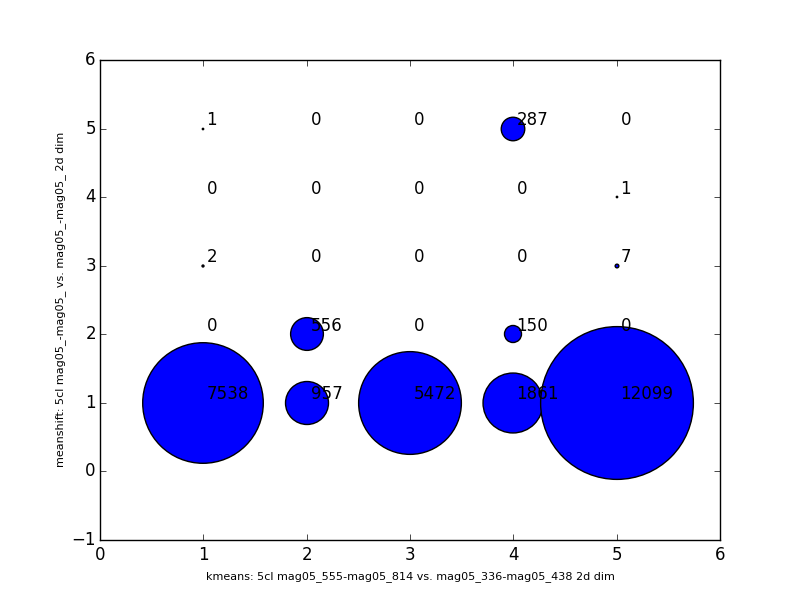
\includegraphics[width=\linewidth]{figs/broad/kmeans-5cl_mag05_555-mag05_814_vs_meanshift-5cl_mag05_-mag05__mag05_-mag05__2ddim_compare}
\caption{Comparison of object cluster assignment between Meanshift and K-Means clusterings.}
\label{fig:BB2dMSKMcomp}
\end{figure}

The axes are the respective clusterings, and the size of the bubble is related to the number of objects that belongs to both clusterings.
It is clear that there is little agreement between the cluster assignment between the two methods. 
Cluster 2, the red branch of objects, is the only cluster where a significant portion of objects were assigned to the same cluster. \textbf{Implication}
K-Means distributes objects far more evenly between clusters, and creates more meaningful segmentation as seen in Figure~\ref{fig:BB2dKM5}.
Due to this comparison, the K-Means segmentation was selected as the optimal clustering for this combination, and was used for the completion of the results.

\paragraph{M83 Locations}

The clusters from the two dimensional clustering show distinct locations in M83.
The branch of red $U - B$ objects found in Cluster 2 of Figure~\ref{fig:BB2dKM5} are objects that lie loosly around the spiral arms.
These objects are generally not found in the concentrated regions of the arms, and lie to the left and right of these areas.
On the whitelight image, these objects appear to be isolated, dim point sources that could be lying behind clouds of dust, in the back of the galaxy, or on their own outside the arm.
\textbf{PB: What could these objects actually be? Young star clusters, clouds, background sources/galaxies?}

The branch of red $V - I$ objects found in Cluster 4 of Figure~\ref{fig:BB2dKM5} are objects that lie primarely in the dense regions of the spiral arms, with a few objects lying in the nucleus, and in the region south of the nucleus.
These objects also appear to be quite dim point sources, or no detection in the whitelight image.
This could mean that the objects are some form of cloud, nebula, or background galaxy. 
These objects are interesting as their $V - I$ colour stretches to values over 3, indicating very red emission. \textbf{PB: is this all true...}

Despite the seemingly arbitrary segmentation of clusters 1 and 3, the objects seem to inhabit different regions of M83.
These two clusters generally trace each others location in the galaxy. 
Cluster 1 is generally confined to the denser regions of the arms, while cluster 3 fills in the areas between the objects in cluster 1.
Cluster 1 objects appear to be bright point sources on the whitelight image, while cluster 3 objects are dim or non-existant.
\textbf{PB: what could these objets be?}.

Interestingly, despite their difference in colour, cluster 5 also traces clusters 1 and 3 around the galaxy.
Cluster 4 objects stay mainly concentrated in the spiral arms, filling in the dense area in the interarm regions.
Cluster 4 objects are not as apparent in the interarm region as clusters 1 and 3, but still appear in denser areas. \textbf{PB: what could these objects be?}

\subsubsection{3-Dimensions}
Three dimensional clustering was performed with the colour combinations found in Table~\ref{tab:BB3dcolours}.

\begin{table*}
\centering
\caption{Broad band colour combinations in three dimensions}
\label{tab:BBcolours}
\begin{tabular}{lllll}
\hline\hline
Base Colour 1 & Base Colour 2 & Colour 1 & Colour 2 & Colour 3 \\
\hline
$U - B$ & $V - I$ & $U - B$ & $B - V$ & $B - I$ \\
$U - V$ & $B - I$ & $U - V$ & $B - V$ & $V - I$ \\
\hline
\end{tabular}
\end{table*}

Both K-Means and Meanshift identified interesting clusters in three dimensions.

\paragraph{K-Means}
Similar to two dimensions, K-Means was able to identify objects that were in specific regions of the colour space.
The optimal K-Means clustering was found at $K=4$ (Figure~\ref{fig:BB3dKM4}), as the score peaked, and the red branch of objects was identified. \textbf{What is the significance of the red branch?}
Figure~\ref{fig:BB3dKMproj} displays the projection of the three dimensional clustering into each of its two dimensional components. 
It is clear that the three dimensional clustering was driven by the $B - I$ vs. $U - B$ distribution, as the clusters were almost completely seperated in that space.
The clusters overlapped extensively in the $B - V$ vs. $U - B$ space. \textbf{PB: Do you know why this would be? Would it be from the range of colour in the B-I dimension?}
This could be a result of the colour distribution in the $B - I$ space, as the range of object colour in this dimension is much larger than in the $B - V$ colour.
This relationship was found through all colour combinations.

\begin{figure*}
\centering
\subfloat[$U - B$ vs. $B - V$ Distribution.]{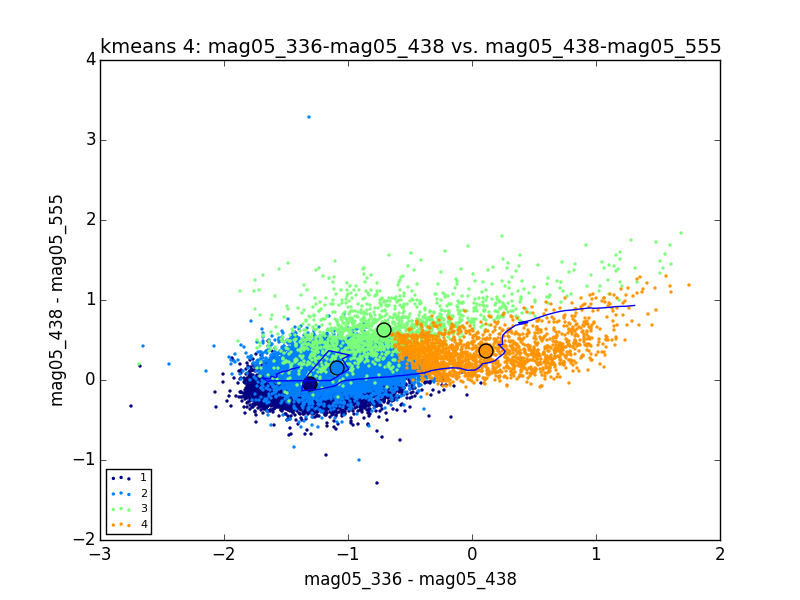
\includegraphics[width=0.5\textwidth]{figs/broad/kmeans_3d_projection_4cl_mag05_336-mag05_438vsmag05_438-mag05_555}\label{fig:BB3dKMprojBV}}
\hfill
\subfloat[$U - B$ vs. $B - I$ Distribution.]{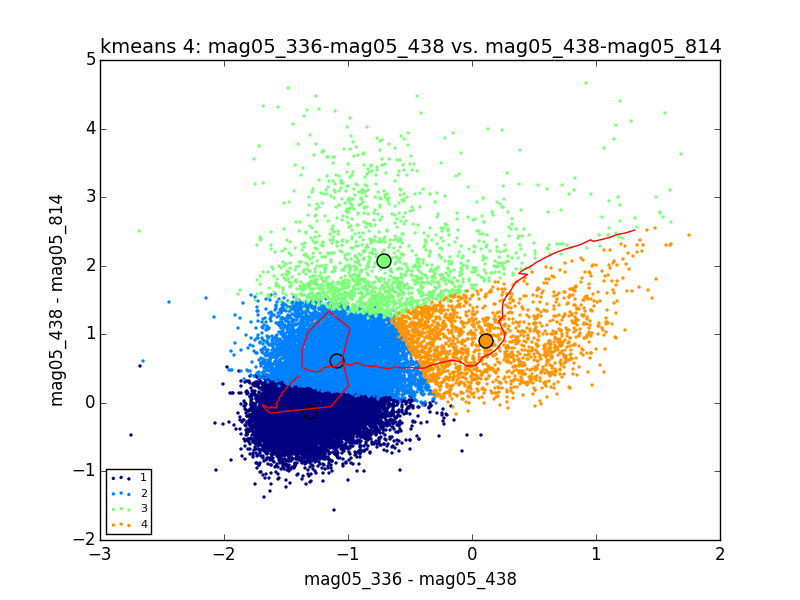
\includegraphics[width=0.5\textwidth]{figs/broad/kmeans_3d_projection_4cl_mag05_336-mag05_438vsmag05_438-mag05_814}\label{fig:BB3dKMprojBI}}
\caption{$U - B$ vs. $B - V$ and $B - I$ projections from three dimensional clustering.}
\label{fig:BB3dKMproj}
\end{figure*}

\begin{figure}[H]
\centering
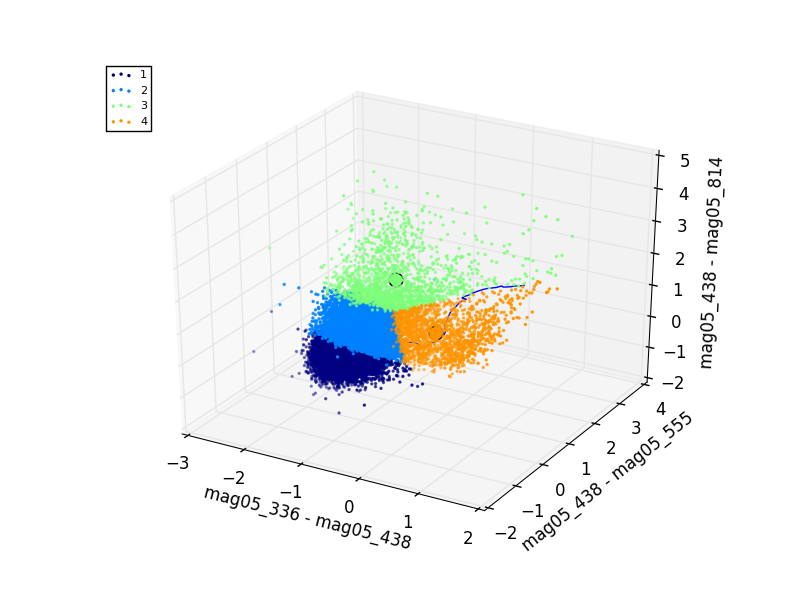
\includegraphics[width=\linewidth]{figs/broad/kmeans_3d_4cl_mag05_336-mag05_438vsmag05_438-mag05_555vsmag05_438-mag05_814}
\caption{Colour-Colour-Colour distribution of the $U - B$, $B - V$, and $B - I$ colours, clustered using K-Means with $K=4$. The colour of each point corresponds to the cluster the point was assigned to. Cluster numbers can be seen in the legend.}
\label{fig:BB3dKM4}
\end{figure}

The three dimensional clustering illustrates how the algorithm is able to identify two distinct branches of objects beyond the dense center of the distribution.
Cluster 4 is a branch of objects that is quite red in both the $U - B$ and $B - V$ colours, but is neutral in the $B - I$ colour.
Cluster 3 is a branch of objects quite blue in the $U - B$ colour, but red in the other two. \textbf{what is the implication of this?}
The algorithm then segments the dense section of the distribution between the bluer and redder objects in the $B - V$ and $B - I$ colours.
These two clusters are not ideal, as the dense portion of the distribution could be argued as the same cluster. 
However, at $K = 3$, the branches were not identified, so the segmentation of the dense region is necessary.
The clusters projected into the base colours can be seen in Figure~\ref{BB3dKM4base}, where the branches of objects are clearly identified.
\textbf{Add cluster statistics table}

\begin{figure}[H]
\centering
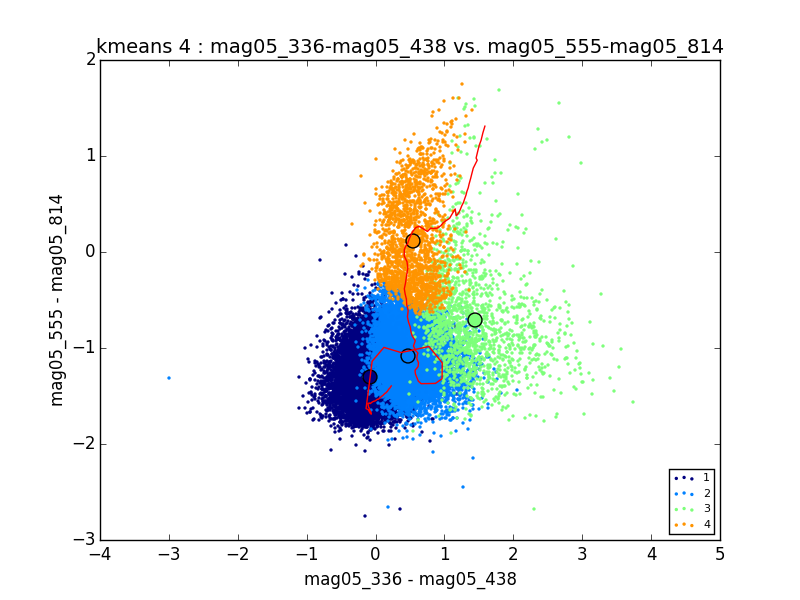
\includegraphics[width=\linewidth]{figs/broad/kmeans_base_color_4cl_mag05_336-mag05_438vsmag05_555-mag05_814}
\caption{Colour-Colour distribution of the $U - B$, and $V - I$ colours, projected from the three dimensional clustering using K-Means with $K=4$. The colour of each point corresponds to the cluster the point was assigned to. Cluster numbers can be seen in the legend.}
\label{fig:BB3dKM4base}
\end{figure}

Similar to the two dimensional clustering, the cluster centers of clusters 1, 2, and 4, match the model colours predicted.
The red branch of objects traces the older stellar population, while clusters 1 and 2 trace the young and intermediate ages of the population.
Cluster 3 is positioned near the loop in the stellar model, however there is a disagreement in the $U - B$ colour.
\textbf{Any other implications of the model matching?}

\paragraph{Meanshift}

Meanshift was also able to produce interesting clusters in three dimensions. 
The optimal clustering was chosen at $h=0.75$ which produced 4 clusters.
This clustering was the peak score, but was not the number of clusters for most intervals of bandwidth.
Most bandwidth values predicted 6 clusters, however, the score and cluster seperation at those intervals was poor.
Figure~\ref{fig:BB3dMS4} shows the three dimensional clustering at $h=0.75$.

\begin{figure}[H]
\centering
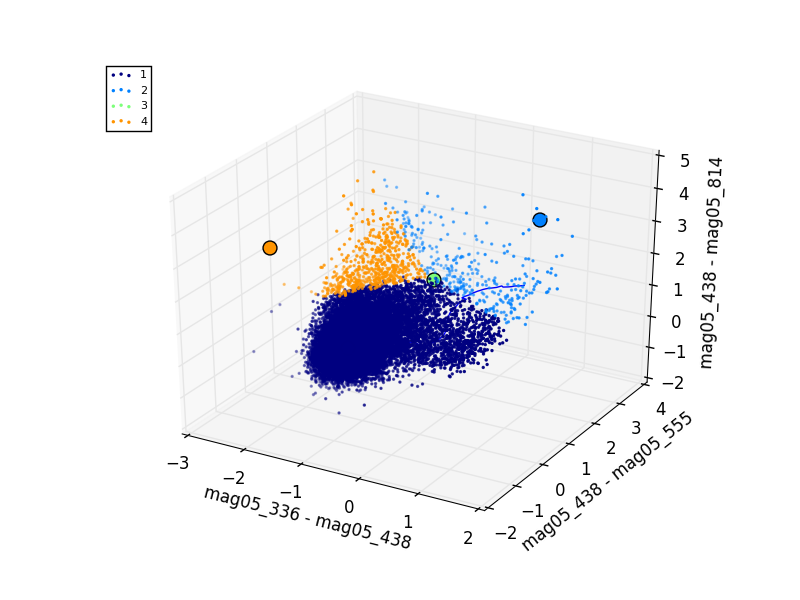
\includegraphics[width=\linewidth]{figs/broad/meanshift_3d_4cl_mag05_336-mag05_438vsmag05_438-mag05_555vsmag05_438-mag05_814}
\caption{Colour-Colour-Colour distribution of the $U - B$, $B - V$, and $B - I$ colours, using Meanshift with $h=0.75$. The colour of each point corresponds to the cluster the point was assigned to. Cluster numbers can be seen in the legend.}
\label{fig:BB3dMS4}
\end{figure}

Meanshift identified two groups of objects that lie above the dense area of the distribution in Figure~\ref{fig:BB3dMS4}.
Figure~\ref{fig:BBMS3d4p} shows the projection into the original space, where the cluster location is easier to identify.
The clustering identified two groups of ojbects which are quite red in the $V - I$ colour, but have different $U - B$ colours. 
Cluster 4 is blue in the $U - B$ colour while Cluster 2 is redder.
This identification highlights Meanshift's ability to find outliers in the distribution, as it does not pick out the large branch of objects that are red in $U - B$.
However, these two clusters combined only hold 3\% of the objects used for clustering.
These clusters would have been considered insignificant, however, they are also found at $h = 0.55$.
This means that the clusters are identified at various bandwidth intervals, which means they are likely significant clusters. 
\textbf{Add cluster statistics table}

\begin{figure}[H]
\centering
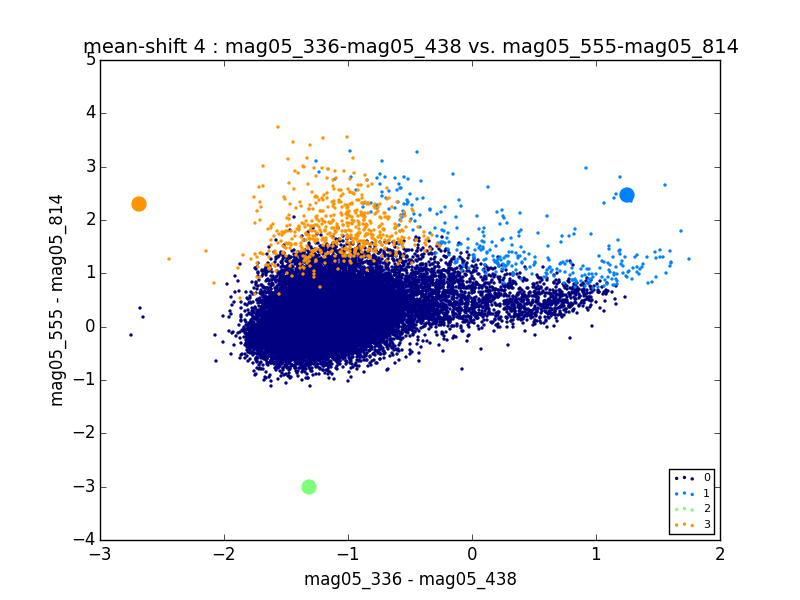
\includegraphics[width=\linewidth]{figs/meanshift_base_color_4cl_mag05_336-mag05_438vsmag05_555-mag05_814}
\caption{Colour-Colour distribution of the $U - B$, and $V - I$ colours, projected from the three dimensional clustering using Meanshift with $h=0.75$. The colour of each point corresponds to the cluster the point was assigned to. Cluster numbers can be seen in the legend.}
\label{fig:BB3dMS4p}
\end{figure}

\paragraph{Cluster Comparison}
Comparing the two clusterings resulted in a similar comparison to the two dimensional clustering.
No significant distribution between clusters was apparent, and all the K-Means clusters were placed in Cluster 1 of the Meanshift clustering.
However, since the three dimensional Meanshift segmentation was more meaningful than the two dimensional clustering, it was kept for further analysis.

\paragraph{M83 Locations}

In the K-Means clustering (Figure~\ref{fig:BB3dKM4p}), clusters 4 and 3 follow similar patterns found in two dimensions.
These clusters are the red $U - B$ branch of objects and the red shelf of $V - I$ objects that span the whole range of $U - B$ colour.
Cluster 4 objects are generally located in the spiral arms, but their location is not concentrated, and they are fanned across the entire width of the arms.
This is in agreement with the cluster that identified the red branch in two dimensions, however, three dimensions seems to include more objects that could be considered redder than the rest of the distribution.
Cluster 3 objects trace cluster 4, but are in the dense regions of the spiral arms, and do not fan out. \textbf{PB: What could these be?}
Clusters 1 and 2 in three dimensions do not provide the same detail as two dimensions as they lump all the objects in the center of the distribution into two groups.
There are no patterns in object location in these two clusters.

The outlying clusters identified by Meanshift in three dimensions are located in interesting areas of M83.
There is almost no overlap between the locations of the objects in these two groups. 
Cluster 2 objects are fanned out through the spiral arms, and in the core of the galaxy.
These objects appear to be dim point sources on the whitelight image, and could be background objects. 
Cluster 4 objects are also found in the spiral arms, however, they are almost only concentrated in the dense areas. 
These objeccts are found in the same regions of the arms as cluster 2, but they are not close to one another. 
This could indicate that these two classes of objects are different physical objects in M83. \textbf{Not sure if this is the right result of their locations}
Lastly, cluster 3, a single object, does not appear to be a meaningful object. It does not seem to be detected in the whitelight image, as it is in an area without a clear, independent point source.
Since this object has very blue colours, it is not clear what it could be, and may be noise. \textbf{Not sure if this is true!}

\subsubsection{Two and Three Dimension Comparison}
Figure~\ref{fig:BB2a3dKMcomp} shows the comparison between the two and three dimensional clusterings.

\begin{figure}[H]
\centering
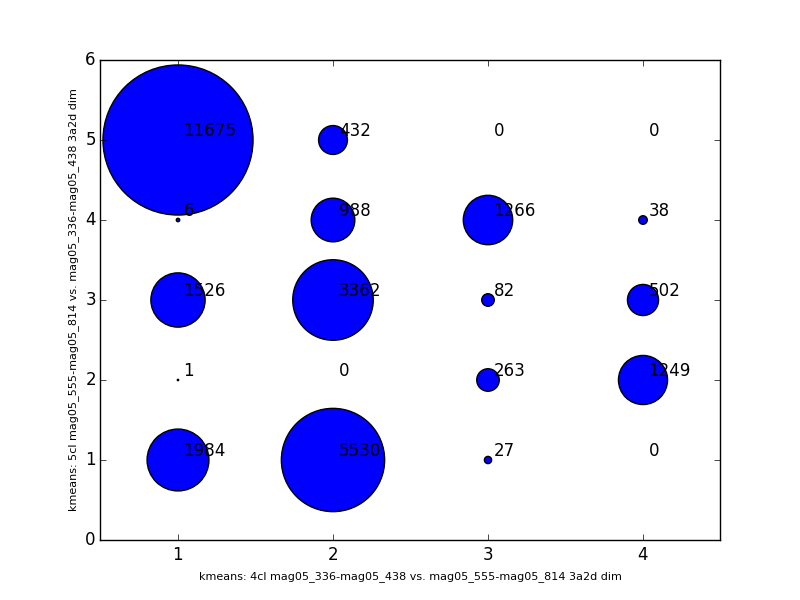
\includegraphics[width=\linewidth]{figs/broad/kmeans-4cl_mag05_336-mag05_438_vs_kmeans-5cl_mag05_555-mag05_814_mag05_336-mag05_438_3a2ddim_compare}
\caption{Comparison of object cluster assignment between K-Means in two dimensions and K-Means in three dimensions.}
\label{fig:BB2dMSKMcomp}
\end{figure}

There is significant overlap in each of the five clusters from the two dimensional clustering.
This shows agreement between the two clusterings for which objects belong in the same cluster. 
It is difficult to compare clusterings with a different number of clusters, but it is clear that Cluster 2 in Figure~\ref{fig:BB3dKM4} is the cluster that is used to add the additional cluster in two dimensions.
With this agreement, it is reasonable to assume that both clusterings are strong, and since the three dimensional clustering had the higher score, it was selected as the optimal clustering.
% ----------------------------------------------

% SUCCESSFUL NAROW BAND CLUSTERINGS ----------------------------------------------
\subsection{U - OII vs. B - V: Successful Clustering}
The U - OII combination was clustered with the B-V, B-I, and V-I colours using Meanshift followed by KMeans. \textbf{More about what we are looking for in this combination}
The $U - OII$ vs. $B - V$ combination was selected for discussion as its K-Means score was the highest in two and three dimensions.
Meanshift did not perform well in two dimensions, but in three dimensions it was able to identify structure in the distribution like K-Means. 

\subsubsection{2-Dimensions}
K-Means performed stronger than Meanshift in two dimensions, and was selected for most of the results. \textbf{Need some introduction to the two dimensional clustering}

\paragraph{Meanshift}
This combination was more sensitive to bandwidth selection than others.
With bandwidth $h=0.2$, $32$ clusters were produced, while $h=0.4$ produced $3$.
Due to this sensitivity, the bandwidth hierarchy was created on much narrower increases in $h$, to produce more meaningful clusters.
After producing the narrow hierarchy, the meanshift algorithm predictad a range of clusters from 3 to 13.
In each clustering, the algorithm did not seem to segment the data significantly, as it produced one large cluster with several smaller ones.
The number of clusters predicted reduced linearly with the bandwidth selected, however, the silhouette score saw a sharp drop at $h = 0.33$, which produced 8 clusters, see Figure ~\ref{fig:UOII2dMS}. 
This clustering segmented the data into three main groups.
Cluster 1 was the densist region of the distribution, and clusters 2 and 5 were were two "arms" in the distribution that spread to the redder areas of both colours.
Despite picking out these two groups, the two arms contained only approximately 5\% of the data. 
Additionally, the outer areas of the arms were segmented into their own clusters. 
These clusters are not meaningful as these objects would have similar properties to each arm.
This segmentation was the strongest two dimensional Meanshift candidate. 
However, since it was still poor, the two dimensional Meanshift clustering was not considered for the rest of the analysis. 

\begin{figure}
\centering
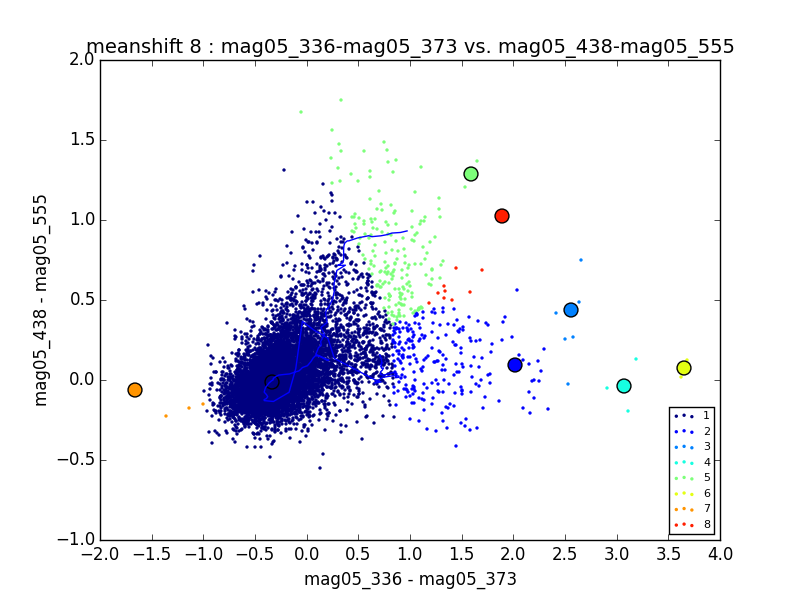
\includegraphics[width=\linewidth]{figs/successful/meanshift_color_8cl_mag05_336-mag05_373vsmag05_438-mag05_555}
\caption{Colour-Colour distribution of the $U-O_{2}$ and B-V colours, clustered using Meanshift with $h=0.33$. The colour of each point corresponds to the cluster the point was assigned to. Cluster numbers can be seen in the legend.}
\label{fig:UOII2dMS}
\end{figure}

\paragraph{K-Means}
The K-Means algorithm produced more reliable results, as it produced clusters of relatively similar sizes.
The silhouette score elbowed at $K=5$, and was selected as the optimal clustering, see Figure~\ref{fig:UOII2dKM5}.
At $K=5$ K-Means segmented the data based on integer colour values, and identified the section of data that was significantly red in the U-OII colour.
The centers of clusters 3, 4, and 5 align well with the model colours.
These clusters identify different ages of the the model stellar population. However, clusters 1 and 2 do not align well with the model, despite identifying seperate parts of the distribution.
\textbf{Add cluster statistics here}

\begin{figure}
\centering
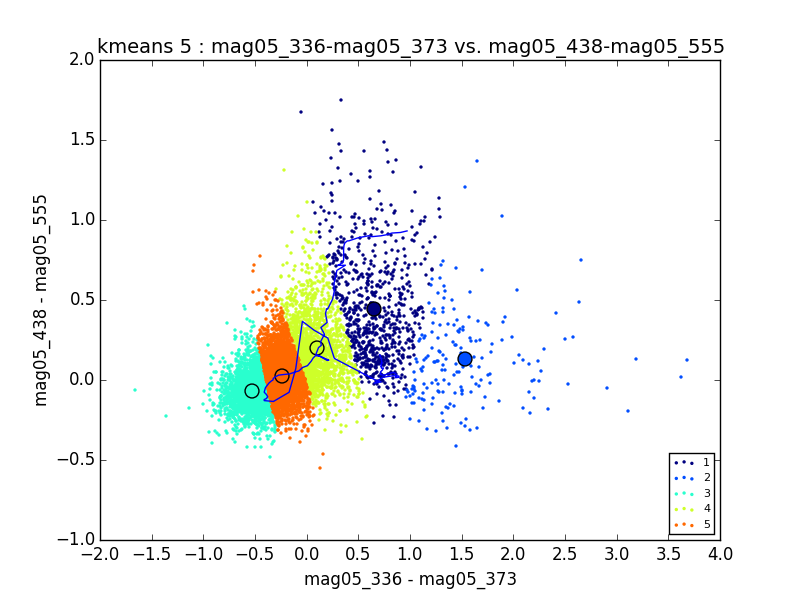
\includegraphics[width=\linewidth]{figs/successful/kmeans_color_5cl_mag05_336-mag05_373vsmag05_438-mag05_555}
\caption{Colour-Colour distribution of the $U-O_{2}$ and B-V colours, clustered using K-Means with $K=5$. The colour of each point corresponds to the cluster the point was assigned to. Cluster numbers can be seen in the legend.}
\label{fig:UOII2dKM5}
\end{figure}

\paragraph{M83 Locations}
\textbf{Need help identifying these objects}
The K-Means clustering was the only segmentation considered on M83, as Meanshift's segmentation was not meaningful.
Cluster 2, the red branch, seemed to be a combination of dim point sources and objects in the back of the galaxy or behind clouds.
A significant portion of cluster 1 objects were found in the core of the galaxy.
The remainder of the objects were distributed throughout the areas surrounding dense regions in the spiral arms, and consisted of bright point sources, and point sources behind clouds or in the back of the galaxy. \textbf{Not sure what the significance of that is since they are red in both colours}
Cluster 3, the objects blue in both colours, are consentrated in the dense regions of the spiral arms.
The few objects that are located in the core are concentrated in the very center, and there are no objects located in the dust lanes between the core and the spiral arm.
Cluster 5 objects are located in the dense regions of the spiral arms, but are not concentrated in the centers of these areas like the objects in cluster 3.
Similar to cluster 5, cluster 3 objects are located sparsly along the dense regions of the spiral arms, and seem to trace the position of the objects in cluster 3. 

\subsubsection{3-Dimensions}

Following the initial clustering, the colours were each broken down into a combination of the OII band and each other band.
The colours used in three dimensions were U-OII, OII-B, and OII-V.

The performance in three dimensions was stronger for all clustering parameters.
The clustering algorithms were able to identify a large branch of objects that was red in the U-OII colour, and very blue in the other two colours, see Figure ~\ref{fig:UOIIKM3d}.
This branch was identified at all values of K, and most values of h.
The added complexity of three dimensions removed the restrictions of only using two dimensions, and allowed the algorithms to cluster the distributions more accurately.

\paragraph{Meanshift}

The optimal meanshift clustering was not as apparent in three dimensions.
The bandwidth did not converge at a number of clusters, or the score.
However, a weak plateau was found when 6 clusters were produced, at $h = 0.62$.
This bandwidth value was the point before a steep drop in the relation between bandwidth and score, and was selected for the optimal clustering.
Figure~\ref{UOII3dMS6} shows the three dimensional clustering. 
The three dimensional clustering was driven by the $O_{2} - B$, and $O_{2} - V$ colours equally, contrary to the pattern found in the broad band clustering.
This means that despite the different range in colours, both colours had attributes to add to the distribution, and the objects in this narrow band have elements in both broad bands. 
\textbf{Not sure if that is the implication}. 

\begin{figure}
\centering
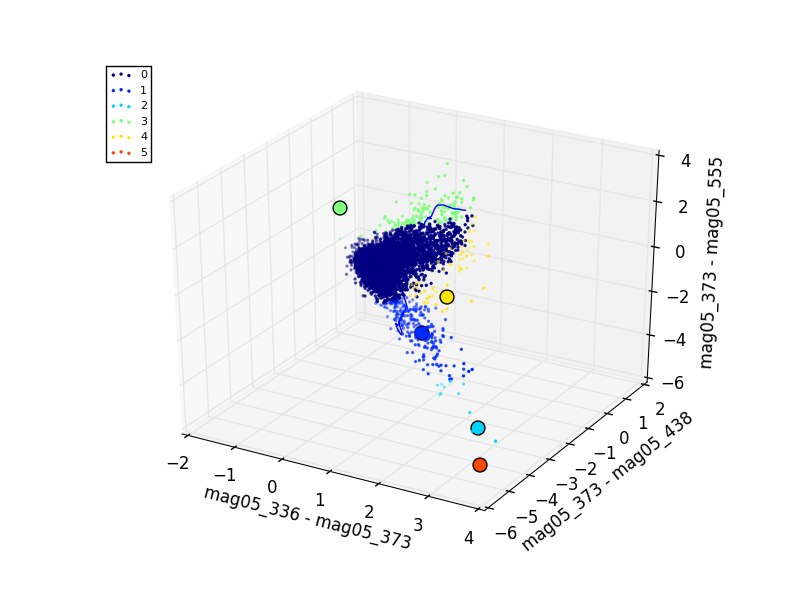
\includegraphics[width=\linewidth]{figs/successful/meanshift_3d_6cl_mag05_336-mag05_373vsmag05_373-mag05_438vsmag05_373-mag05_555}
\caption{Colour-Colour-Colour distribution of the $U-O_{2}$, $O_{2} - B$, and $O_{2} - V$ colours, clustered using Meanshift with $h=0.62$. The colour of each point corresponds to the cluster the point was assigned to. Cluster numbers can be seen in the legend.}
\label{fig:UOII3dMS6}
\end{figure}

Meanshift identified groups of objects that did not lie in the dense center of the distribution.
Several clusters can be seen that are well defined in three dimensions, but are not apparent in the two dimensional projection (Figure~\ref{fig:UOII3dMSbase}).
The clusters that seem obvious in three dimensions overlap significantly in two dimensions.
However, this clustering is stronger than the two dimensional clustering.
\textbf{Need more implications}

\begin{figure}
\centering
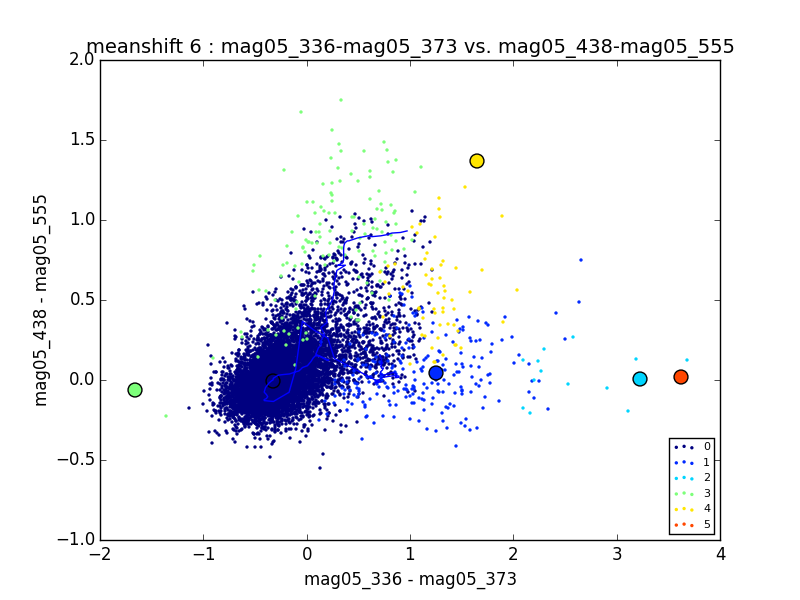
\includegraphics[width=\linewidth]{figs/successful/meanshift_base_color_6cl_mag05_336-mag05_373vsmag05_438-mag05_555}
\caption{Colour-Colour distribution of the $U-O_{2}$, and $B - V$ colours, projection from the three dimensional clustering using Meanshift with $h=0.62$. The colour of each point corresponds to the cluster the point was assigned to. Cluster numbers can be seen in the legend.}
\label{fig:UOII3dMS6}
\end{figure}

\paragraph{K-Means}
The K-Means algorithm was superior to meanshift for picking out evenly sized groups in all combinations, however, it was not able to pick out some of the detail lying in the groups of outlier data. 
The score peaked at $K=3$ (Figure~\ref{UOIIKM3d}), which was much higher than any other value of $K$.
This was caused by the clear segmentation of the branch of blue objects in three dimensions.
When projected into two dimensions, the successful segmentation of K-Means can be seen, as it identifies both branches of red objects, and the dense area around zero, see Figure ~\ref{fig:UOIIKM2d}.
Additionally, all three cluster centers align with segments of the model colours.
Cluster 1 is a branch of young stars, and each cluster progresses in the age of the stellar population.
This pattern is even more pronounced for higher values of $K$, but the clustering accuracy is reduced significantly as $K$ increases.

\begin{figure}
\centering
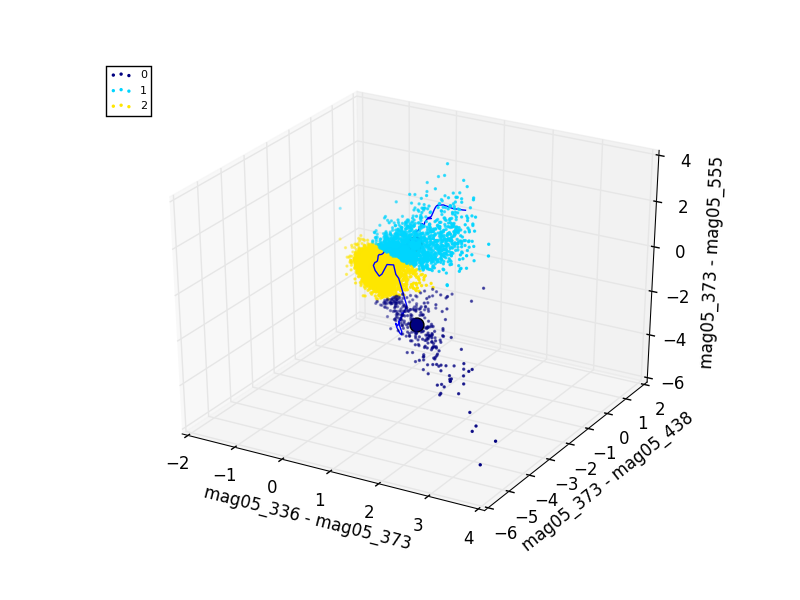
\includegraphics[width=\linewidth]{figs/successful/kmeans_3d_3cl_mag05_336-mag05_373vsmag05_373-mag05_438vsmag05_373-mag05_555}
\caption{Colour-Colour-Colour distribution of the $U-O_{2}$, $O_{2}-B$, and $O_{2}-V$ colours, clustered using K-Means with $K=3$. The colour of each point corresponds to the cluster the point was assigned to. Cluster numbers can be seen in the legend.}
\label{fig:UOIIKM3d}
\end{figure}

\begin{figure}
\centering
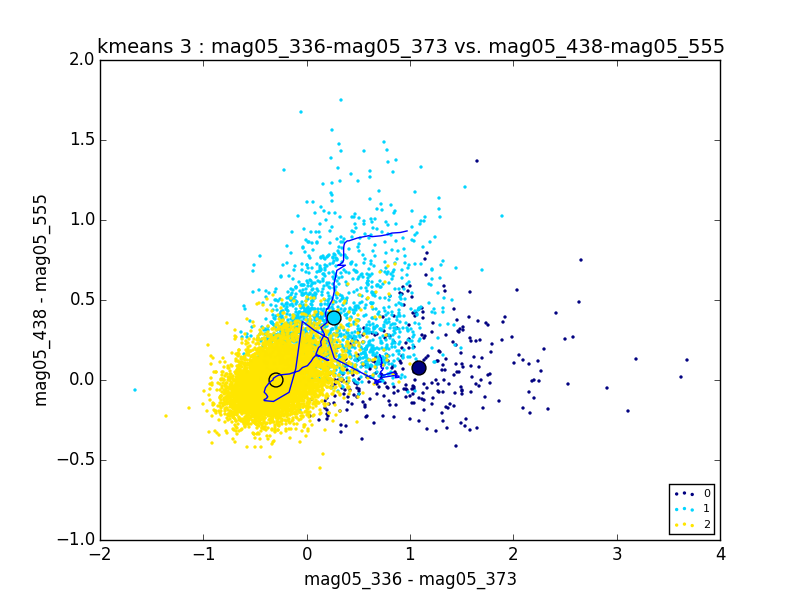
\includegraphics[width=\linewidth]{figs/successful/kmeans_base_color_3cl_mag05_336-mag05_373vsmag05_438-mag05_555}
\caption{Colour-Colour distribution of the $U-O_{2}$ and B-V colours, projected from the 3D clustering using K-Means with $K=3$. The colour of each point corresponds to the cluster the point was assigned to. Cluster numbers can be seen in the legend.}
\label{fig:UOIIKM2d}
\end{figure}

\paragraph{M83 Locations}
Clusters 1 and 2 were almost entirely objects in the back of the galaxy or behind clouds.
The objects in cluster 3 were located in the densist areas of the spiral arms.
These locations agree with the two dimensional clustering, however, clusters 1 and 2 are much more pronounced in three dimensions.
The three dimensional clustering was stronger as the objects in each cluster were not similar to the objects in the other two clusters, which was not the case in two dimensions.
% ----------------------------------------------

% UNSUCCESSFUL NARROW BAND CLUSTERING ----------------------------------------------
\subsection{$O_{3}$-V vs. U - B: Unsuccessful Clustering}
The $O_{3}$-V colour was clustered with the U - B colour in two dimensions and the U-$O_{3}$, and B-$O_{3}$ colours in three dimensions.
The clustering methods were not successful at identifying structure in this combination in both two and three dimensions.
The results were driven by the colour distribution.
In two dimensions, the majority of the objects had $O_{3} - V$ colours between $-0.5$ and $+0.5$. 
This did not give the clustering algorithms enough information to use, and caused the poor segmentation.

\subsubsection{2-Dimensions}

\paragraph{Meanshift}
The Meanshift clustering does not seem to provide meaningful segmentation.
The meanshift parameters do not display the same patterns as other combinations. 
The Meanshift score did not plateau at any number of clusters, and the large center cluster contained almost all of the objects in each segmentation.
Meanshift identified the branch of blue objects at all bandwidth levels, but as the number of clusters increases the clusters are forced into segmenting the blue objects, not the rest of the distribution.
At $h=0.2$, 8 clusters are produced (Figure~\ref{fig:OIIIV2dMS}), and Meanshift identified many clusters in the blue branch, and a larger cluster of objects that are quite red in the U-B cluster.
This clustering results in a peak in the score.
Despite identifying different parts of the distribution, the algorithms performance does not match the patterns of other combinations.
Additionally, the cluster centers do not match the model colours. 
Meanshift was not able to segment the stellar population based on age, as it had in other combinations.

\begin{figure}
\centering
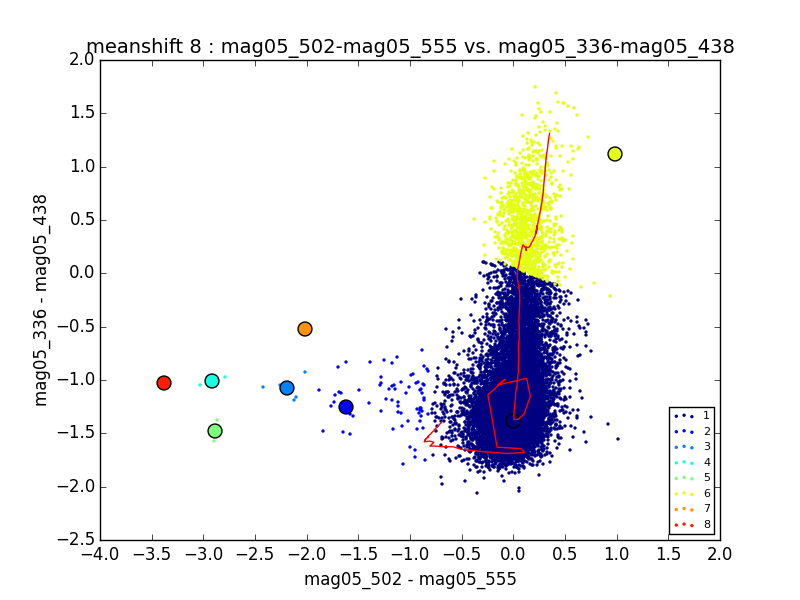
\includegraphics[width=\linewidth]{figs/unsuccessful/meanshift_color_8cl_mag05_502-mag05_555vsmag05_336-mag05_438}
\caption{Colour-Colour distribution of the $O_{3}$-V and U - B colours, clustered using Meanshift with $h=0.28$. The colour of each point corresponds to the cluster the point was assigned to. Cluster numbers can be seen in the legend.}
\label{fig:OIIIV2dMS}
\end{figure}

\paragraph{K-Means}
The K-Means two dimensional clustering segmented the data into sections of U-B colour.
As K increased, K-Means was able to identify a branch of objects that are bluer in both colours.
The segmentation in the colour-colour space translated into the U-B vs B CMD. 
Each clustering segmented the CMD by U-B colour, and the cluster of bluer objects appears to be a group of objects bright in the U band with a brightest B magnitude of approximately 25.
The K-Means score begins to plateau at K=4, however K=5 has a slightly higher score than the rest of the plateau as this is the first clustering to identify the branch of bluer objects.
Despite the plateau, the clustering scores are not as high as other combinations, and the segmentation appears to be arbitrary.
K-Means optimal clustering was $K=4$ (Figure~\ref{fig:OIIIV2dKM}), which did not identify the clear branch of blue objects.
Despite the poor segmentation, the cluster centers aligned well with the colour models, tracing them through the distribution.
The clusters selected different ages of the stellar population, but the segmentation was still poor, and a result of the distribution. 

\begin{figure}
\centering
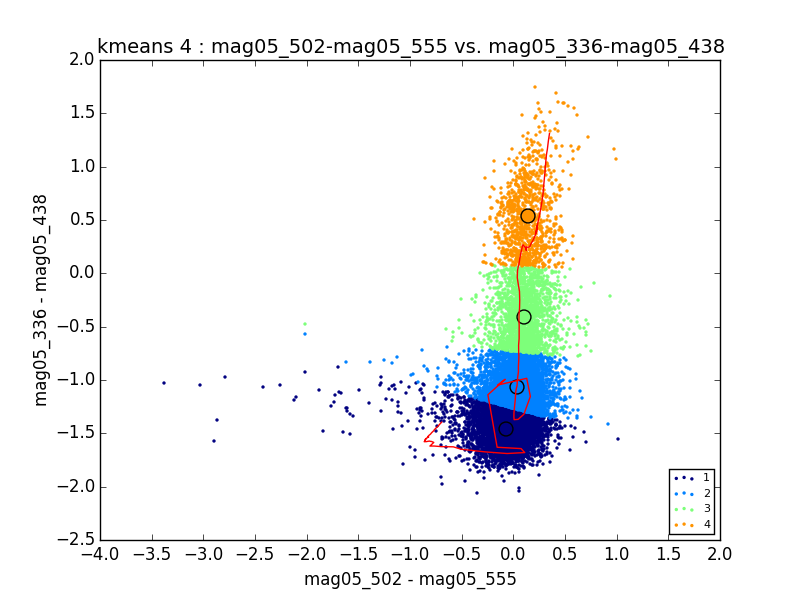
\includegraphics[width=\linewidth]{figs/unsuccessful/kmeans_color_4cl_mag05_502-mag05_555vsmag05_336-mag05_438}
\caption{Colour-Colour distribution of the $O_{3}$-V and U - B colours, clustered using K-Means with $K=4$. The colour of each point corresponds to the cluster the point was assigned to. Cluster numbers can be seen in the legend.}
\label{fig:OIIIV2dKM}
\end{figure}

\paragraph{Cluster Comparison}
Figure~\ref{fig:OIIIV2dcomp} shows the comparison between the optimal K-Means and Meanshift clusterings.
There is little agreement between the two methods on which clusters the objects belong to.

\begin{figure}[H]
\centering
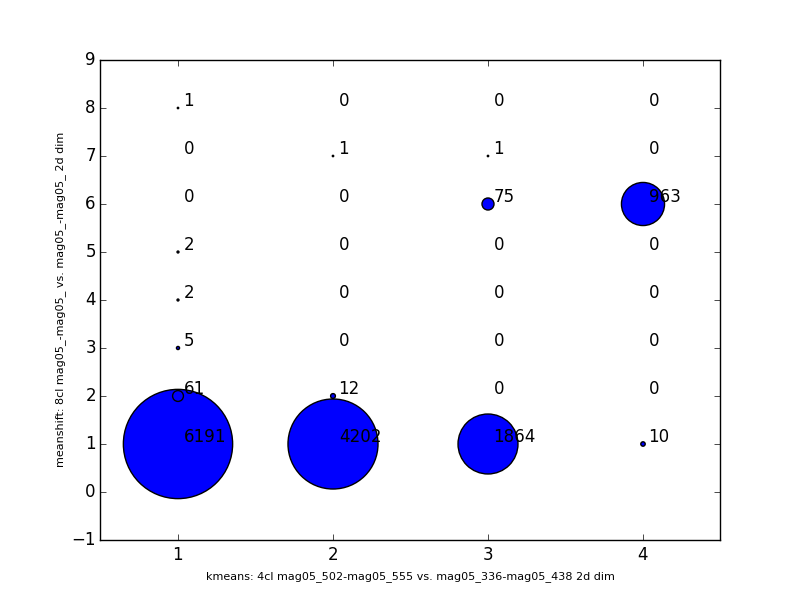
\includegraphics[width=\linewidth]{figs/unsuccessful/kmeans-4cl_mag05_502-mag05_555_vs_meanshift-8cl_mag05_-mag05__mag05_-mag05__2ddim_compare}
\caption{Comparison of object cluster assignment between K-Means at K=4 and Meanshift at h=0.28 in two dimensions.}
\label{fig:OIIIV2dcomp}
\end{figure}

The only clusters that agree are cluster four in K-Means and six in Meanshift.
These clusters are the red branch of objects in the $O_{3}$-V colour.
The Meanshift clusters that segment the blue branch are quite small, and K-Means is unable to identify those objects as independent clusters.

\paragraph{M83 Locations}
The K-Means clusters did not show distinct patterns through M83.
Since the segmentation does not pick out specific structure in the distribution, it was unlikely that the spatial relationships were as significant as other colour combination.
This was confirmed as there did not seem to be a difference in location between the objects in cluster 1 and 4 in Figure~\ref{fig:OIIIV2dKM}.
The objects Meanshift clusters 2, 3, 4, 5, 7, and 8 identify objects that are spread out through the spiral arms, without any objects in the core.
Despite their interesting locations, these clusters combined consisted of less than 1\% of the data in the combination, and the other clusters did not create meaningful patterns.

\subsubsection{3-Dimensions}
The three dimensional distribution displays more structure than two dimensions.
Two clear features are visible, a branch of objects that are red in the U-$O_{3}$ colour, and neutral in the rest, and a second branch of objects that are blue in the $O_{3}$-V colour, red in the B-$O_{3}$ colour, and neutral in the U-$O_{3}$ colour.

\paragraph{Meanshift}
The Meanshift score plateaued clearly at 7 clusters. There is a large drop in score between 5 and 7 clusters, and both clusterings were able to identify both branches.
Additionally, Meanshift was able to identify sub-clusters within the blue branch of objects, that are objects with extremely blue colours, see Figure ~\ref{fig:OIIIVMS3d}.
The Meanshift clustering was more effective than K-Means, as it did not segment the dense area after it had identified each branch.
The clustering with 5 clusters was chosen as the optimal clustering as the clustering with 7 clusters divided the red branch in two, causing significant overlap in the two and three dimensional spaces.
This segmentation is not as strong as the other combinations as the optimal clustering combines two branches of objects.
The result is the combination of objects that clearly have very different colours.

\begin{figure}
\centering
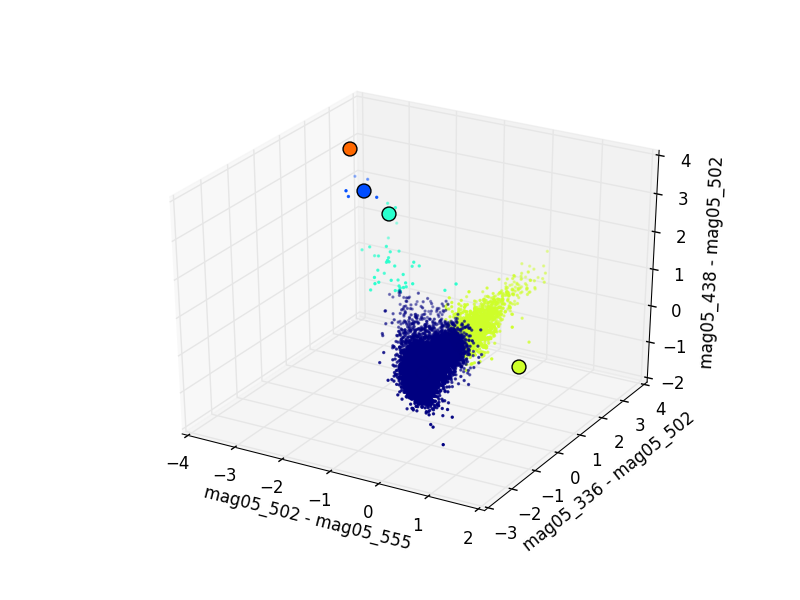
\includegraphics[width=\linewidth]{figs/meanshift_3d_color_5cl_mag05_502-mag05_555vsmag05_336-mag05_502vsmag05_438-mag05_502}
\caption{Colour-Colour-Colour distribution of the U-$O_{3}$, B-$O_{3}$, and $O_{3}$-V colours, clustered using Meanshift with $h=0.5992$. The colour of each point corresponds to the cluster the point was assigned to. Cluster numbers can be seen in the legend.}
\label{fig:fig:OIIIVMS3d}
\end{figure}

\paragraph{K-Means}
At all values of K, K-Means is able to identify the first branch of objects. However, it is not until K=6 that the algorithm was able to identify the second branch as its own cluster, see Figure~\ref{fig:OIIIVKM3d}.
By this point, the algorithm has segmented the dense area of the distribution by its U-$O_{3}$ colour.
When projected into two dimensions, there is significant overlap between the clusters that were segmented by colour, and the first branch of objects does not seem to be its own cluster in two dimensions.
The score at K=6 causes a slight peak, which shows the effect of picking out both branches of objects.
However, the score is still significantly lower than the clusterings that do not identify these branches.

\begin{figure}
\centering
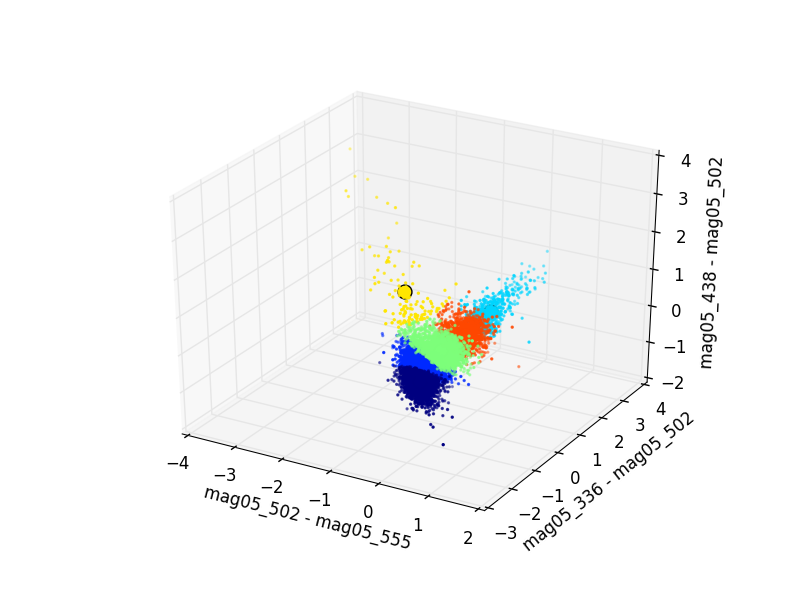
\includegraphics[width=\linewidth]{figs/kmeans_3d_color_6cl_mag05_502-mag05_555vsmag05_336-mag05_502vsmag05_438-mag05_502}
\caption{Colour-Colour-Colour distribution of the U-$O_{3}$, B-$O_{3}$, and $O_{3}$-V colours, clustered using K-Means with $K=6$. The colour of each point corresponds to the cluster the point was assigned to. Cluster numbers can be seen in the legend.}
\label{fig:fig:OIIIVKM3d}
\end{figure}

\paragraph{M83 Locations}
After investigating each clustering on the whitelight image, most segmentations did not identify sets of objects that were located in specific areas of the galaxy.
Cluster 4 of the strongest Meanshift clustering identified objects that were located in the less dense regions of the spiral arms of M83.
This cluster isolated the branch of red objects in the colour distribution.
Additionally, this cluster was clearly defined in the CMD and split the objects at colour 0.
The largest cluster in the blue branch of objects picked isolated objects in the spiral arm, with only one object located in the nucleus.
All of these objects appear to be background galaxy objects or objects behind clouds, as few of the objects appeared in the whitelight image.
The other two clusters that segmented the blue branch were also objects that appear to be background or covered by clouds, indicating that these objects are quite bright in the $O_{3}$ band, and not in the V band.

